\subsection{连通分支}

对拓扑空间 X 的给定一点 x，X 中含有 x 的诸连通子集之并是连通的（第 1 目，命题 2）；因而它是 X 中含有 x 的最大连通子集。

定义 3. 拓扑空间 X 的一点的分支（或连通分支）是 X 中含有该点的最大连通子集。X 的子集 A 的诸分支是 A 的诸点相对于子空间 A 的分支。

若空间连通，则每一点的分支都是全空间。若空间 X 使得对 X 的每一对点 \((x, y)\) 都存在含有 x 与 y 的连通集，则 X 连通。

如果 X 的每一点的分支仅由该点组成，就称空间 X 是全不连通的。如果 X 的子空间 A 是全不连通的，就称 X 的子集 A 是全不连通集。

离散空间是全不连通的，但应注意不要混淆这两个概念；例如，我们将在第四章，§ 2，第 5 目看到，有理直线不是离散空间，却是全不连通的。

\pandocbounded{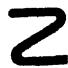
\includegraphics[keepaspectratio]{images/part001_10033d49.jpg}}

既开又闭的集合含有其每一点的分支，由此，一点的分支含于既开又闭且含有该点的诸集合之交。然而，一点的分支未必等于这个交（参见习题 9 及第二章，§ 4，第 4 目，命题 6）。

命题 9. 拓扑空间 X 中任一点的分支是闭集。关系“y 属于 x 的分支”是 X 上的一个等价关系 R\{x, y\}，其等价类就是 X 的诸分支。商空间 X/R 是全不连通的。

命题的第一部分是定义 3 与连通集的闭包连通（第 1 目，命题 1）这一事实的直接推论。由于有公共点的诸连通集之并是连通的（第 1 目，命题 2），关系 R 是传递的，因而是等价关系（因为它显然是自反且对称的），且 x 关于 R 的等价类就是 x 的分支。尚须证明 X/R 是全不连通的。设 \(f: X \to X/R\) 是典范映射，F 是 X/R 中含有至少两个不同点的闭集；F 的逆像 \(\overline{f}^{1}(F)\) 在 X 中是闭的、关于 R 是饱和的，且含有 X 的至少两个不同分支，因而不连通。于是存在 X 中两个非空闭集 B, C，使得 \(B \cap C = \varnothing\) 且 \(B \cup C = \overline{f}^{1}(F)\)。\(\overline{f}^{1}(F)\) 中任一点 x 在 \(\overline{f}^{1}(F)\) 中的分支与 x 在 X 中的分支相同（由 R 的定义），因此在 \(\overline{f}^{1}(F)\) 中既开又闭的 B 与 C 关于 R 是饱和的。于是 \(f(B)\) 与 \(f(C)\) 在 X/R 中是闭的，且 \(f(B) \cup f(C) = F\)，\(f(B) \cap f(C) = \varnothing\)；这表明 F 不连通，从而 X/R 是全不连通的。

命题 10. 在积空间 \(\mathbf{X} = \prod_{i\in J}\mathbf{X}_i\) 中，\(x = (x_i)\) 在 \(\mathbf{X}\) 中的分支是诸 \(x_i\) 在因子 \(\mathbf{X}_i\) 中的分支之积。

这个积集合是连通的（第 4 目，命题 8）。反之，若 A 是 X 的含有 x 的连通子集，则 \(\mathrm{pr}_{i}(A)\) 是含有 x 的连通集（第 2 目，命题 4）；由于 \(A \subset \prod_{i} \mathrm{pr}_{i}(A)\)，可见 A 含于诸 \(x_{i}\) 的分支之积中。

